\documentclass[12pt,letterpaper]{article}
\usepackage[utf8]{inputenc} %Spanish input
\usepackage[T1]{fontenc} % Use 8-bit encoding that has 256 glyphs
\usepackage[spanish, es-tabla]{babel} % Selecciona el español para palabras introducidas automáticamente, p.ej. "septiembre" en la fecha y especifica que se use la palabra Tabla en vez de Cuadro
\usepackage{fullpage}
\usepackage[top=2cm, bottom=4.5cm, left=2.5cm, right=2.5cm]{geometry}
\usepackage{amsthm,amsfonts,amssymb,amscd}
\usepackage[fleqn]{amsmath}
\usepackage{lastpage}
\usepackage{enumerate}
\usepackage[inline]{enumitem}
\usepackage[cmintegrals,cmbraces]{newtxmath}
\usepackage{fancyhdr}
\usepackage{mathrsfs}
\usepackage{xcolor}
\usepackage{array,multirow,stackengine,graphicx,wrapfig}
\usepackage{cellspace}
\setlength{\cellspacetoplimit}{5pt}
\setlength{\cellspacebottomlimit}{5pt}
\usepackage{hhline}
\usepackage{listings}
\usepackage{hyperref}
\usepackage{titletoc,tocloft}
\usepackage{mathtools}
\usepackage{float,subfig}
\usepackage[linguistics,edges]{forest} % for trees
\setlength{\cftsubsecindent}{2cm}
\setlength{\cftsubsubsecindent}{4cm}
\dottedcontents{section}[1.5em]{}{1.3em}{.6em}
\usepackage[nodisplayskipstretch]{setspace}
\setstretch{.5}
\usepackage[export]{adjustbox}
\usepackage{pdflscape}
\setstackEOL{\\}

\usepackage{pgfgantt}
\newcommand\Dganttbar[4]{%
  \ganttbar{#1}{#3}{#4}\ganttbar[inline,
  bar label font=\footnotesize]
  {#2}{#3}{#4}
}


\graphicspath{ {./imgs/} } %Drawing the background pic
\usepackage{tikz}
\newcommand{\tikzmark}[1]{\tikz[baseline,remember picture] \coordinate (#1) {};}
\usetikzlibrary{positioning}
\usetikzlibrary{shadows,arrows.meta} % For adding edges label
\usetikzlibrary{calc}
\usepackage{eso-pic}
\AddToShipoutPictureBG{%
\begin{tikzpicture}[remember picture, overlay]
\node[opacity=.15, inner sep=0pt]
    at(current page.center){
\includegraphics[scale=1.5]{logo-ugr2}};
\end{tikzpicture}%
}

\numberwithin{equation}{section} % Number equations within sections (i.e. 1.1, 1.2, 2.1, 2.2 instead of 1, 2, 3, 4)
\numberwithin{figure}{section} % Number figures within sections (i.e. 1.1, 1.2, 2.1, 2.2 instead of 1, 2, 3, 4)
\numberwithin{table}{section} % Number tables within sections (i.e. 1.1, 1.2, 2.1, 2.2 instead of 1, 2, 3, 4)

\forestset{ %Formatting my tree
.style={for tree={parent anchor=south, child anchor=north,align=center,base=bottom,where n children=0{tier=word}{}}},
background tree/.style={for tree={text opacity=0.2,draw opacity=0.2,edge={draw opacity=0.2}}}
}
%\forestset{%
%  declare dimen register={gap},
%  gap'=20mm,
%  declare dimen register={lbox width},
%  lbox width=(\textwidth-2*\forestregister{gap})/3,
%  rbox/.style = {draw=blue!80!black, fill=blue!20, rounded corners},
%  lbox/.style = {align/.wrap pgfmath arg={@{}p{##1 pt}@{}}{(lbox_width)}},
%}


\hypersetup{%
    colorlinks=true,
    linkcolor=[rgb]{0.2, 0.3, 0.5},
    urlcolor=black,
    citecolor=black,
    linkbordercolor={0 0 1}
}


\renewcommand\lstlistingname{Graphics}
\renewcommand\lstlistlistingname{Graphics}
\def\lstlistingautorefname{IG.}

\newcommand{\horrule}[1]{\rule{\linewidth}{#1}} % Create horizontal rule command with 1 argument of height
\definecolor{codegreen}{rgb}{0,0.6,0}
\definecolor{codegray}{rgb}{0.5,0.5,0.5}
\definecolor{codepurple}{rgb}{0.58,0,0.82}
\definecolor{backcolour}{rgb}{0.95,0.95,0.92}

\lstdefinestyle{bash}{
    backgroundcolor=\color{backcolour},
    commentstyle=\color{codegreen},
    keywordstyle=\color{magenta},
    numberstyle=\tiny\color{codegray},
    stringstyle=\color{codepurple},
    basicstyle=\ttfamily\footnotesize,
    breakatwhitespace=false,
    breaklines=true,
    keepspaces=true,
    numbers=left,
    numbersep=5pt,
    showspaces=false,
    showstringspaces=false,
    showtabs=false,
    tabsize=2
}\setlength{\parindent}{0.0in}
\setlength{\parskip}{0.05in}
\lstset{style=bash}

% Edit these as appropriate
\newcommand\course{Ingeniería Informática }
\newcommand\hwnumber{1}                  % <-- homework number
\newcommand\NetIDa{Brian,}           % <-- NetID of person #1
\newcommand\NetIDb{Sena Simons}

\pagestyle{fancyplain}
\headheight 35pt
\lhead{\NetIDa}
\lhead{\NetIDa\\\NetIDb}                 % <-- Comment this line out for problem sets (make sure you are person #1)
\chead{\textbf{\Large Satisfacción de Restricciones}}
\rhead{\course \\ \today}
\lfoot{\scriptsize\LaTeX}
\cfoot{\hyperlink{Indice}{Volver al índice}}
\rfoot{\small\thepage}
\headsep 1.5em

\renewcommand*\contentsname{Índice}

\author{Brian Sena Simons} % Nombre y apellidos

\date{\normalsize\today} % Incluye la fecha actual


\begin{document}
\begin{titlepage}
\begin{figure}[H]
    \vspace{-1.3cm}
    \begin{center}
        
\includegraphics[width=0.75\textwidth]{Etsiit}
    \end{center}
\end{figure}
\vspace{1.3cm}
\centering
\normalfont \normalsize
    \textsc{\textbf{Técnicas de Sistemas Inteligentes 2021-2022} \\ Grado en Ingeniería Informática \\ Universidad de Granada} \\ [25pt] % Your university, school and/or department name(s)
    \horrule{0.5pt} \\[0.4cm] % Thin top horizontal rule
    \huge Memoria Práctica 2 \\ % The assignment title
    \horrule{2pt} \\[0.5cm] % Thick bottom horizontal rule

\begin{minipage}{0.4\textwidth}
    \begin{flushleft}\large
        \emph{Autor:} \\
        \vspace{.15cm}
        Brian Sena Simons.
    \end{flushleft}
\end{minipage}
\begin{minipage}{0.4\textwidth}
     \begin{flushright}\large
         \emph{Grupo: } \\
         3ºA Subgrupo A2
    \end{flushright}
\end{minipage}
\end{titlepage}

\doublespacing
\hypertarget{Indice}{}
\tableofcontents
\newpage
\section{Ejercicio 1}
En este apartado tenemos que diseñar una representación del problema de asignación
de monedas para un importe dado. Para ello he optado por utilizar un vector
con dónde cada posición es una cantidad de moneda y otro vector de igual
tamaño que para cada posición tiene el valor de esa moneda. De esta manera
podemos alcanzar un importe N como la suma de las cantidades por sus valores.
\par
La implementación inicial del apartado a) no impone ninguna restricción sobre
el orden de las monedas y/o si se debe minimizar la cantidad. Por lo que como
podemos verificar con la tabla, el tiempo de cómputo que utiliza ``MiniZinc''
crece de forma exponencial por la explosión combinatoria de soluciones sobre
que cantidad de cada moneda puede utilizar para resolver el problema, ya que
habría miles de combinaciones según el tamañó de importe.

\begin{table}[H]
    \centering
    \small
\begin{tabular}{|rccc|}
\hline
\multicolumn{4}{|c|}{\textbf{Tabla 1.1: Apartado a).}}                                                                                                                                     \\ \hline
\multicolumn{1}{|c|}{\textbf{Importe}} & \multicolumn{1}{c|}{\textbf{Solución Encontrada}} & \multicolumn{1}{c|}{\textbf{Total de Soluciones}} & \textbf{Runtime (Segundos)} \\ \hline
\multicolumn{1}{|r|}{\textbf{0.17}}    & \multicolumn{1}{c|}{17}                                   & \multicolumn{1}{c|}{28}                                  & 0.18                        \\ \hline
\multicolumn{1}{|r|}{\textbf{1.43}}    & \multicolumn{1}{c|}{143}                                  & \multicolumn{1}{c|}{17952}                               & 1.319                       \\ \hline
\multicolumn{1}{|r|}{\textbf{2.35}}    & \multicolumn{1}{c|}{235}                                  & \multicolumn{1}{c|}{150824}                              & 10.8634                     \\ \hline
\multicolumn{1}{|r|}{\textbf{4.99}}    & \multicolumn{1}{c|}{499}                                  & \multicolumn{1}{c|}{6224452}                             & 427.12                      \\ \hline
\end{tabular}
\end{table}

\begin{table}[H]
    \small
    \centering
\begin{tabular}{|rccc|}
\hline
\multicolumn{4}{|c|}{\textbf{Tabla 1.2: Apartado b).}}                                                                                                                                     \\ \hline
\multicolumn{1}{|c|}{\textbf{Importe}} & \multicolumn{1}{c|}{\textbf{Solución Encontrada}} & \multicolumn{1}{c|}{\textbf{Total de Soluciones}} & \textbf{Runtime (Segundos)} \\ \hline
\multicolumn{1}{|r|}{\textbf{0.17}}    & \multicolumn{1}{c|}{17}                                   & \multicolumn{1}{c|}{28}                                  & 0.159                       \\ \hline
\multicolumn{1}{|r|}{\textbf{1.43}}    & \multicolumn{1}{c|}{44}                                   & \multicolumn{1}{c|}{284}                                 & 1.352                       \\ \hline
\multicolumn{1}{|r|}{\textbf{2.35}}    & \multicolumn{1}{c|}{36}                                   & \multicolumn{1}{c|}{162}                                 & 0.206                       \\ \hline
\multicolumn{1}{|r|}{\textbf{4.99}}    & \multicolumn{1}{c|}{101}                                  & \multicolumn{1}{c|}{4366}                                & 6.352                       \\ \hline
\end{tabular}
\end{table}

\begin{table}[H]
    \small
    \centering
\begin{tabular}{|rccc|}
\hline
\multicolumn{4}{|c|}{\textbf{Pregunta 1: Apartado c).}}                                                                                                                                    \\ \hline
\multicolumn{1}{|c|}{\textbf{Importe}} & \multicolumn{1}{c|}{\textbf{Solución Encontrada}} & \multicolumn{1}{c|}{\textbf{Total de Soluciones}} & \textbf{Runtime (Segundos)} \\ \hline
\multicolumn{1}{|r|}{\textbf{0.17}}    & \multicolumn{1}{c|}{3}                                   & \multicolumn{1}{c|}{15}                                  & 0.162                       \\ \hline
\multicolumn{1}{|r|}{\textbf{1.43}}    & \multicolumn{1}{c|}{5}                                   & \multicolumn{1}{c|}{40}                                  & 0.156                       \\ \hline
\multicolumn{1}{|r|}{\textbf{2.35}}    & \multicolumn{1}{c|}{4}                                   & \multicolumn{1}{c|}{32}                                  & 0.171                       \\ \hline
\multicolumn{1}{|r|}{\textbf{4.99}}    & \multicolumn{1}{c|}{8}                                   & \multicolumn{1}{c|}{94}                                  & 0.722                       \\ \hline
\end{tabular}
\end{table}

Con los resultados obtenidos empiricamente he llegado a la conclusión que MiniZinc
converge antes cuántas más restricciones impones sobre las variables libres. En
otras palabras, el tiempo de cómputo para el apartado ``a'' es inviable para
valores de importe muy elevados. Si estuvieramos hablando de importe de miles
de millones de euros igual tardaría cuestión de días, ya que sigue como
un esquema de fuerza bruta empezando por el valor de menor restricción.
\par
Incluso si utilizaramos las versiones ``b'' y ``c'' vemos que aún es notable
el crecimiento del tiempo de cómputo pero a menor medida. Una posible solución
para este problema para importes muy elevados consiste en utilizar un criterio
de elección de variables al revés de como hace MiniZinc. En pocas palabras,
la idea clave sería empezar por aquellas monedas con mayor valor hasta que
nos pasemos del importe, retroceder y probar con la siguiente mayor. De esta
manera nos aseguramos que la solución obtenida será la óptima y además se
encontrará en muchas menos iteraciones.

\begin{figure}[H]
    \centering
    \subfloat{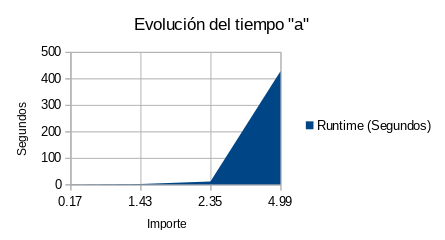
\includegraphics[scale=.6]{TiempoA.png}}
    \subfloat{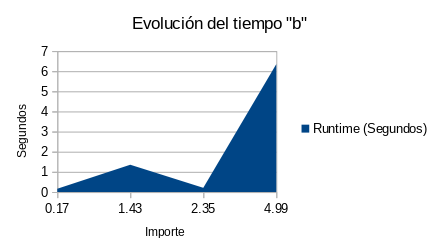
\includegraphics[scale=0.6]{TiempoB.png}}\\
    \subfloat{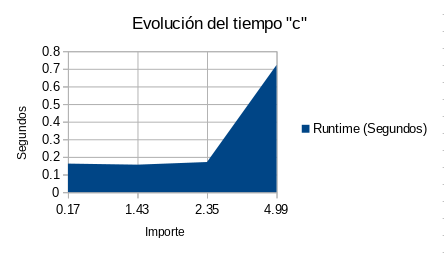
\includegraphics[scale=0.6]{TiempoC.png}}
    \caption{Evolución del tiempo de cómputo según restricciones.}
\end{figure}

\section{Ejercicio 2}
Tenemos que planificar los horarios de un conjuntos de asignaturas acorde
con las restricciones de horas semanales, de disponibilidad de los profesores
y de días asignados para cada asignatura entre otras. Los horarios obtenidos
para este ejercicio son los siguientes:

\begin{table}[H]
    \centering
    \small
\subfloat{
\begin{tabular}{|cccccc|}
\hline
\multicolumn{6}{|c|}{\textbf{Asignación de horarios Instituto}}                                                                                                                                                                               \\ \hline
\multicolumn{1}{|c|}{\textbf{Horario}}  & \multicolumn{1}{c|}{\textbf{Lunes}} & \multicolumn{1}{c|}{\textbf{Martes}} & \multicolumn{1}{c|}{\textbf{Miercoles}} & \multicolumn{1}{c|}{\textbf{Jueves}} & \multicolumn{1}{c|}{\textbf{Viernes}} \\ \hline
\multicolumn{1}{|c|}{\textbf{08:00:00}} & \multicolumn{1}{c|}{A4}             & \multicolumn{1}{c|}{A4}              & \multicolumn{1}{c|}{A8}                 & \multicolumn{1}{c|}{A5}              & A5                                    \\ \hline
\multicolumn{1}{|c|}{\textbf{09:00:00}} & \multicolumn{1}{c|}{A4}             & \multicolumn{1}{c|}{A4}              & \multicolumn{1}{c|}{A8}                 & \multicolumn{1}{c|}{A5}              & A5                                    \\ \hline
\multicolumn{1}{|c|}{\textbf{10:00:00}} & \multicolumn{1}{c|}{A9}             & \multicolumn{1}{c|}{A7}              & \multicolumn{1}{c|}{A6}                 & \multicolumn{1}{c|}{A2}              & A6                                    \\ \hline
\multicolumn{1}{|c|}{\textbf{11:00:00}} & \multicolumn{1}{c|}{Recreo}         & \multicolumn{1}{c|}{Recreo}          & \multicolumn{1}{c|}{Recreo}             & \multicolumn{1}{c|}{Recreo}          & Recreo                                \\ \hline
\multicolumn{1}{|c|}{\textbf{12:00:00}} & \multicolumn{1}{c|}{A1}             & \multicolumn{1}{c|}{A1}              & \multicolumn{1}{c|}{A3}                 & \multicolumn{1}{c|}{A3}              & A2                                    \\ \hline
\multicolumn{1}{|c|}{\textbf{13:00:00}} & \multicolumn{1}{c|}{A1}             & \multicolumn{1}{c|}{A1}              & \multicolumn{1}{c|}{A3}                 & \multicolumn{1}{c|}{A3}              & A7                                    \\ \hline
\end{tabular}} \\
\subfloat{
\begin{tabular}{|cccccc|}
\hline
\multicolumn{6}{|c|}{\textbf{Asignación de horarios Instituto}}                                                                                                                                                          \\ \hline
\multicolumn{1}{|c|}{\textbf{Horario}}  & \multicolumn{1}{c|}{\textbf{Lunes}} & \multicolumn{1}{c|}{\textbf{Martes}} & \multicolumn{1}{c|}{\textbf{Miercoles}} & \multicolumn{1}{c|}{\textbf{Jueves}} & \textbf{Viernes} \\ \hline
\multicolumn{1}{|c|}{\textbf{08:00:00}} & \multicolumn{1}{c|}{A4}             & \multicolumn{1}{c|}{A4}              & \multicolumn{1}{c|}{A8}                 & \multicolumn{1}{c|}{A5}              & A5               \\ \hline
\multicolumn{1}{|c|}{\textbf{09:00:00}} & \multicolumn{1}{c|}{A4}             & \multicolumn{1}{c|}{A4}              & \multicolumn{1}{c|}{A8}                 & \multicolumn{1}{c|}{A5}              & A5               \\ \hline
\multicolumn{1}{|c|}{\textbf{10:00:00}} & \multicolumn{1}{c|}{A9}             & \multicolumn{1}{c|}{A7}              & \multicolumn{1}{c|}{A6}                 & \multicolumn{1}{c|}{A2}              & A6               \\ \hline
\multicolumn{1}{|c|}{\textbf{11:00:00}} & \multicolumn{1}{c|}{Recreo}         & \multicolumn{1}{c|}{Recreo}          & \multicolumn{1}{c|}{Recreo}             & \multicolumn{1}{c|}{Recreo}          & Recreo           \\ \hline
\multicolumn{1}{|c|}{\textbf{12:00:00}} & \multicolumn{1}{c|}{A1}             & \multicolumn{1}{c|}{A1}              & \multicolumn{1}{c|}{A3}                 & \multicolumn{1}{c|}{A3}              & \textcolor{red}{A7}               \\ \hline
\multicolumn{1}{|c|}{\textbf{13:00:00}} & \multicolumn{1}{c|}{A1}             & \multicolumn{1}{c|}{A1}              & \multicolumn{1}{c|}{A3}                 & \multicolumn{1}{c|}{A3}              & \textcolor{red}{A2}               \\ \hline
\end{tabular}
}
\end{table}

Apenas he obtenido 2 soluciones, que son simétricas ya que semánticamente son
exactamente lo mismo, el mismo profesor da las mismas clases pero intercambiadas
de hora. Este es uno de los problemas que nos podemos encontrar con MiniZinc.
Que aunque haya encontrado una solución no sabe diferenciar entre soluciones
simétricas y esto puede ser un problema, en el ejercicio 5 fue mucho más notable
por el increible aumento del tiempo de cómputo.
\par
Por ello se recomienda tomar iniciativas para saber diferenciar cuando estamos
ante una solución simétrica e intentar obviar su exploración. En cualquier
caso, en este ejercicio quizás por la implementación apenas he obtenido
1 solución y otra simétrica a ella. En el ejercicio 5 se vuelve hablar del tema.

\section{Ejercicio 3}
En este ejercicio tenemos que resolver un problema lógico de las cinco casas,
quiénes viven en ellas, con qué animales, cuáles son sus bebidas y cuáles son
sus profesiones. Para ello he optado por tomar el camino de asignar una
variable para cada característica perteneciente a un individuo. Es decir,
si el brasileño bebe whiskey, entonces brasileño = whiskey = 10/10.
\par
La idea a partir de esto es ir definiendo una a una las igualdades provenientes
del enunciado. De tal manera que, en menos de 0.1 segundos, he podido fácilmente
obtener que \textbf{la cebra pertenece al gallego} y el \textbf{andaluz bebe agua}.

\section{Ejercicio 4}
Este sin duda fue el ejercicio más dificil para mi, la representación de lo
que es la concurrencia fue un tremendo reto. Sin embargo, tras leer el manual
oficial de MiniZinc, y replantear el ejercicio miles de veces he logrado obtener
resultados optimistas.
\par
El ejercicio nos impone una tabla de tareas, nos indica que tenemos tres trabajadores
tales que cada uno tiene un tiempo asignado para poder completar tal tarea, y
entre ellos pueden trabajar concurrentemente. Además, ciertas actividades
tienen que realizarse antes de las demás.
\par
Para ello he utilizado un vector de tareas con valores que especifican
cuando empieza cada tarea. (vector[1] = 0 -> Tarea 1 empieza día 0).
Luego además tengo un vector de tareas con sus respectivas duraciones, una matriz
con los tiempos y otra que representa las tareas, que trabajador la hace y cuando.
Además he utilizado funcionalidades de MiniZinc como es ``alternative'' y
``disjunctive'' que me ayudan a decidir que tarea realizar y con que trabajador y
evitar solapamiento. El resultado obtenido se verifica en el siguiente diagrama:

\begin{figure}[H]
\begin{center}
\begin{ganttchart}[
  vgrid,
            x unit=0.7cm,
            y unit title=0.8cm,
            y unit chart=1.5cm,
  hgrid,
  expand chart=1\textwidth,
  vrule/.style={very thick, blue},
  vrule label font=\bfseries
]{0}{13}
\gantttitle{Días}{14} \\
\ganttbar[inline=false]{Trabajador 1}{1}{3}
\ganttbar[inline]{A}{0}{3}
\ganttbar[inline]{D}{4}{5}
\ganttbar[inline]{B}{6}{8}
\ganttbar[inline]{I}{9}{10} \\
\ganttbar[inline=false]{Trabajador 2}{6}{7}
\ganttbar[inline]{G}{6}{7}
\ganttbar[inline]{E}{8}{9}
\ganttbar[inline]{C}{10}{10} \\
\ganttbar[inline=false]{Trabajador 3}{4}{8}
\ganttbar[inline]{H}{4}{8}
\ganttbar[inline]{F}{9}{10}
\ganttvrule[
  vrule/.append style={red, thin},
  ]{día 4}{3}
 \ganttvrule[
  vrule/.append style={gray, thin},
  ]{día 6}{5}
\ganttvrule{día 11}{10}

\end{ganttchart}
\end{center}
\caption{Diagrama para 3 trabajadores.}
\end{figure}

Como podemos observar en nuestro diagrama de Gantt, vemos que forzosamente empezamos por la actividad A, y a
continuación disparamos dos actividades de forma simúltanea a parti del día 4. En el día 6 tenemos dónde se
alcanza la máxima eficiencia con los 3 trabajadores activos. Esta es la mejor combinación que nos indica Minizinc
en alrededor de 12 segundos. \textbf{El tiempo mínimo para terminar todas las tareas es de 11 días.}

\begin{figure}[H]
\begin{center}

\begin{ganttchart}[
  vgrid,
            x unit=0.7cm,
            y unit title=0.8cm,
            y unit chart=1.5cm,
  hgrid,
  expand chart=1\textwidth,
  vrule/.style={very thick, blue},
  vrule label font=\bfseries
]{0}{13}
\gantttitle{Días}{14} \\
\Dganttbar{Trabajador 1}{A}{0}{1}
\ganttbar[inline]{B}{2}{2}
\ganttbar[inline]{D}{3}{4}
\ganttbar[inline]{H}{5}{5}
\ganttbar[inline]{G}{6}{6}\\
\Dganttbar{Trabajador 2}{C}{3}{3}
\ganttbar[inline]{E}{4}{5}
\ganttbar[inline]{I}{6}{6}\\
\Dganttbar{Trabajador 3}{F}{4}{4}\\
\Dganttbar{Trabajador 4}{A}{0}{1}
\ganttbar[inline]{B}{2}{2}
\ganttbar[inline]{I}{6}{6}
\ganttvrule[
  vrule/.append style={red, thin},
  ]{día 2}{1}
 \ganttvrule[
  vrule/.append style={blue, thin},
  ]{día 7}{6}

\ganttvrule[
  vrule/.append style={brown, thin},
  ]{día 11}{10}

\end{ganttchart}
\end{center}
\caption{Diagrama para 4 trabajadores.}
\end{figure}

Ya en el caso de emplear un cuarto trabajador que reduce el tiempo de ejecución de una tarea
en 2 días para todas tareas de igual o más de 3 días de duración el resultado es de \textbf{7 días}.
Esto es debido a que puede llegar mucho antes a alcanzar la máxima eficiencia entre los trabajadores
y además permite mayor flexibilidad a la hora de elegir qué trabajador hace qué tarea obteniendo así
menores tiempos.

\section{Ejercicio 5}
Para este ejercicio disponemos de un código de python que nos genera un grafo de N nodos y M aristas sobre
una semilla S. Estos datos debemos pasarlos a MiniZinc y colorear, ojo, a las aristas no a los nodos.
Antes de empezar con el código realizé algunos ejercicios sencillos sobre un grafo de 4 nodos y conexiones
secuenciales del 1 al 4... luego probé con los casos esquinas como lo son los grafos completos... y llegué a la
conclusión obvia que el máximo número de colores sería equivalente al número de nodos que hay en nuestro grafo,
ya que sería el máximo número de aristas salientes posibles de un nodo concreto.
\par
Con esta información podemos establecer una cota superior y ayudar a MiniZinc a que converja antes. La implementación
consiste en utilizar un esquema de matriz de adyacencia que se accede mediante los valores que corresponde a la pareja
arista. Cada posición de la matriz que haga falta le asignaremos un color de 1..MAX. Si accedemos a la matriz en la
fila 1 y columna 2, asignamos el mismo valor a fila 2, columna 1. Con esto, con simplesmente hacer uso de la librería
``alldifferent\_except\_0'', por fila,  aseguramos que todas aristas tengan colores diferentes.
Para evitar soluciones simétricas he impuesto que los colores van en orden creciente con
la ayuda de ``value\_precede'' según el manual de MiniZinc.
\begin{table}[H]
    \centering
\begin{tabular}{|l|c|c|}
\hline
\textbf{Tamaño del Grafo} & \textbf{Número de Colores} & \textbf{Runtime (segundos)} \\ \hline
\textbf{N=4, M=6}         & 3                          & 0.161                       \\ \hline
\textbf{N=6, M=15}        & 5                          & 0.161                       \\ \hline
\textbf{N=8, M=28}        & 6                          & 0.159                       \\ \hline
\textbf{N=10, M=45}       & 8                          & 0.172                       \\ \hline
\textbf{N=12, M=66}       & 8                          & 0.175                       \\ \hline
\textbf{N=14, M=91}       & 11                         & 0.192                       \\ \hline
\textbf{N=100, M=4950}    & 75                         & 11.941                      \\ \hline
\textbf{N=125, M=7750}    & 90                         & 30.452                      \\ \hline
\end{tabular}
\end{table}

El ejercicio en si parece bastante escalable en tiempo
de cómputo para el problema de coloreo de aristas en el caso de mi implementación.
Sin embargo, es evidente observar que en complejidad espacial estoy utilizando
una cantidad enorme de memoria. Una pequeña mejora sería modificar la representación
para una matriz triangular y reducir a la mitad el uso de memoria.
\par
De hecho, la razón por la que he parado en N=125, es debido a que con valores
más grandes como \{1000,500,250,200,150\} me he quedado rápidamente sin memoria
y eso que dispongo de 16GB de RAM. Por lo que es evidente, que incluso si utilizaramos
la matriz triangular no sería escalable en esta versión.
Habría que buscar otra implementación.


\end{document}
%------------------------------------------------

\bibliography{citas} %archivo citas.bib que contiene las entradas
\bibliographystyle{plain} % hay varias formas de citar

\end{document}
